% !TeX spellcheck = en_US
\section*{Test run of detrnn.py}

Test report

by E. Marquer, 2018/04/27 Synalp and Université de Lorraine

\subsection{Abstract}

Test to do a complete run, with GPU, of the basic model of DetRNN.

\subsection{Paradigm}

With branch \emph{reimplement}, allocated time 24h, not interactive

Test run of \emph{detrnn.py} with info log output, with \emph{cuda}, for
4 epochs.

With curve auto-plotting, and plot data backup in case of interruption.

\subsubsection{Node}

OAR\_JOB\_ID=1554682 with GPU

Job start time: 2018-04-27 14:11:00

Estimated job stop time: 2018-04-28 14:11:00

Command used:
\lstinline!bash oarsub -q production -p "GPU <> 'NO'" -l "nodes=1,walltime=24:00:00" ~/awd-lstm-lm/rundet.sh!

\subsection{Results}

Total run time for 4 epochs: 5h33

The most rapid progress was during first epoch, with a maximal decrease
of loss of 3/epoch, then the decrease of loss became a constant
0.25/epoch.

\newpage
\subsubsection{Plot}

\begin{figure}[h]
\centering
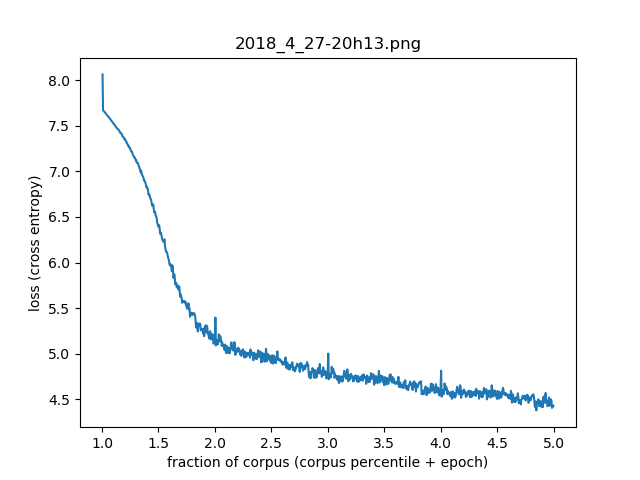
\includegraphics{parts/appendix/reports-gmsnn/docs_esteban-latex/test_reports/2018_4_27-20h13.png}
\caption{plot}
\end{figure}

\subsubsection{Details}

\begin{itemize}
\item
  log
  \href{https://gitlab.inria.fr/emarquer/awd-lstm-lm/blob/reimplement/logs/detrnn2018_4_27-14h11.log}{detrnn2018\_4\_27-14h11.log}
\item
  plot
  \href{https://gitlab.inria.fr/emarquer/awd-lstm-lm/blob/reimplement/plots/2018_4_27-20h13.png}{2018\_4\_27-16h42.png}
\end{itemize}

\subsection{Potential ameliorations \& next steps}

Next step is to test with more epochs, or test the growing model.
